\cotefile{148}
\scanpage{9}
\mspage{3}

B) Courbes \inserted{ell.} anharmoniques de type hexagonal.

La catégorie de ces courbes équivalente : celle des hexagones orientés,
i.e. des torseurs $S$ sous
\[
\begin{aligned}
\mathbb Z/6\mathbb Z&\simeq\mu_6(\mathbb C)\simeq
\text{groupe des}\\
&\qquad\qquad\text{unités \inserted{\unsure{alg.}} de }Q\left(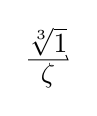
\begin{tikzpicture}[baseline=(rad.base)]
\node[inner sep=0pt] (rad) {$\sqrt[3]{1}$};
\draw[line width=.35pt] ([yshift=-1pt]rad.south west) -- ([yshift=-1pt]rad.south east) -- ++(-.025,.06);
\node[below=2pt,inner sep=0pt] at (rad.south) {$\zeta$};
\end{tikzpicture}\right)\\
&\simeq\text{groupe des unités \unsure{\begin{tikzpicture}[x=.04em,y=-.04em,line cap=round,line join=round,baseline=-.15ex]
\draw[line width=.35pt] (0,14) .. controls (5,14) and (13,8) .. (11,3)
 .. controls (10,0) and (7,0) .. (6,3)
 .. controls (3,8) and (8,12) .. (23,14);
\end{tikzpicture}}}\\
&\qquad\text{\uline{\unsure{\deleted{de}}}}\quad \deleted{\mathbb Z[\zeta]\unsure{=}\mathbb Z[T]/}\\
&\qquad \mathbb Z[\zeta]=\mathbb Z[T]/(1+T+T^2)\\
&\qquad (\zeta=\exp 2i\pi/\unsure{3})
\end{aligned}
\]

\figure{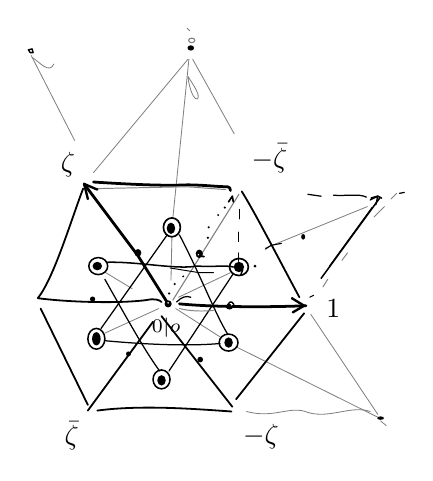
\begin{tikzpicture}[x=.012cm,y=-.012cm,line cap=round,line join=round]
% Exposed pale construction strokes and their interrupted ends.
\draw[gray,line width=.3pt] (172,921) -- (218,1011);
\draw[gray,line width=.3pt] (173,923) .. controls (181,928) and (191,941) .. (196,930);
\draw[gray,line width=.3pt] (238,1045) -- (338,925);
\draw[gray,line width=.3pt] (343,925) -- (387,1004);
\draw[gray,line width=.3pt] (339,925) -- (322,1093);
\draw[gray,line width=.3pt] (338,943) .. controls (342,950) and (352,963) .. (348,967)
  .. controls (342,968) and (338,947) .. (338,943);
\draw[gray,line width=.3pt] (321,1114) -- (320,1159);
\draw[gray,line width=.3pt] (251,1151) -- (279,1168);
\draw[gray,line width=.3pt] (325,1189) -- (372,1219);
\draw[gray,line width=.3pt] (390,1230) -- (539,1304);
\draw[gray,line width=.3pt] (250,1215) -- (307,1189);
\draw[gray,line width=.3pt] (328,1177) -- (383,1151);
\draw[gray,line width=.3pt] (468,1195) -- (539,1301);
\draw[gray,line width=.3pt] (400,1298) .. controls (430,1306) and (446,1291) .. (465,1299)
  .. controls (488,1306) and (511,1291) .. (531,1298);
\draw[gray,line width=.3pt] (420,1125) -- (528,1081);
% Outer sides: retain the gaps at the exposed junctions.
\draw[line width=.65pt] (227,1062) .. controls (215,1093) and (196,1157) .. (179,1178)
  .. controls (209,1182) and (263,1184) .. (294,1180)
  .. controls (303,1178) and (308,1180) .. (310,1182);
\draw[line width=.65pt] (182,1189) -- (232,1291);
\draw[line width=.65pt] (242,1297) .. controls (288,1291) and (342,1295) .. (384,1298);
\draw[line width=.65pt] (389,1285) -- (461,1194);
\draw[line width=.65pt] (395,1065) .. controls (410,1089) and (437,1142) .. (456,1177);
\draw[line width=.65pt] (310,1197) -- (385,1293);
\draw[line width=.65pt] (232,1297) -- (301,1203);
\draw[gray,line width=.4pt] (322,1180) -- (392,1068);
% Heavy top edge and its visible downward terminal curl.
\draw[line width=1pt] (238,1055) .. controls (285,1058) and (315,1059) .. (337,1058)
  .. controls (354,1058) and (369,1060) .. (380,1060)
  .. controls (382,1060) and (383,1062) .. (383,1064);
\draw[gray,line width=.35pt] (240,1062) -- (337,1060) -- (378,1063);
\node[above,inner sep=0pt,font=\scriptsize] at (382,1054) {\unsure{}};
% Two exposed directed heavy radii, drawn with their visible wings.
\draw[line width=1pt] (317,1184) -- (285,1133) -- (228,1057);
\draw[line width=.85pt] (232,1073) -- (228,1057) -- (242,1063);
\draw[line width=1pt] (329,1184) .. controls (359,1187) and (413,1188) .. (463,1186);
\draw[line width=.85pt] (448,1178) -- (461,1186) -- (449,1193);
% Inner triangular strokes, retaining their irregular paths.
\draw[line width=.45pt] (316,1111) -- (246,1210);
\draw[line width=.45pt] (329,1111) .. controls (351,1153) and (367,1195) .. (380,1216);
\draw[line width=.45pt] (250,1223) .. controls (292,1227) and (338,1229) .. (372,1226);
\draw[line width=.45pt] (250,1158) .. controls (272,1197) and (293,1235) .. (308,1255);
\draw[line width=.45pt] (318,1255) -- (386,1152);
\draw[line width=.55pt] (252,1140) .. controls (285,1139) and (326,1148) .. (347,1144)
  .. controls (365,1145) and (380,1143) .. (386,1145);
\draw[line width=.35pt] (319,1146) -- (350,1151) -- (365,1151);
% Individually visible marks on the dotted oblique and vertical strokes.
\foreach \x/\y/\r in {318/1173/1.3,324/1163/1.3,333/1155/1.1,359/1114/1.3,360/1103/1.2,370/1090/1.1,377/1082/1.3}{\fill (\x,\y) circle[radius=\r];}
\draw[line width=.6pt] (381,1076) -- (385,1070) -- (386,1076);
\draw[line width=.35pt] (393,1084) -- (393,1094) (392,1108) -- (392,1118) (391,1130) -- (391,1139);
% Exposed right-hand extension, parallel strokes, and short marks.
\draw[line width=.45pt] (465,1068) -- (479,1070);
\draw[line width=.45pt] (492,1069) .. controls (506,1070) and (519,1067) .. (527,1071);
\draw[line width=.6pt] (532,1072) -- (539,1070) -- (543,1072);
\draw[line width=.55pt] (479,1157) -- (541,1072);
\draw[line width=.45pt] (488,1144) -- (533,1082);
\draw[gray,line width=.35pt] (481,1166) -- (486,1158) (501,1138) -- (507,1130) (535,1092) -- (546,1081) (553,1073) -- (559,1067);
\draw[line width=.45pt] (562,1067) -- (567,1066);
\draw[line width=.4pt] (420,1126) -- (426,1122) -- (437,1120);
\draw[line width=.4pt] (467,1177) -- (471,1175);
% Six irregular ringed points with dark centers.
\draw[line width=.6pt] (321,1103) ellipse[x radius=9,y radius=10];
\fill (320,1104) ellipse[x radius=4.5,y radius=6];
\draw[line width=.6pt] (392,1145) ellipse[x radius=10,y radius=9];
\fill (392,1145) circle[radius=5.5];
\draw[line width=.55pt] (381,1225) ellipse[x radius=10,y radius=9];
\fill (381,1225) ellipse[x radius=4.5,y radius=5.5];
\draw[line width=.55pt] (310,1264) ellipse[x radius=9,y radius=10];
\fill (310,1265) ellipse[x radius=4.5,y radius=5.5];
\draw[line width=.55pt] (241,1221) ellipse[x radius=9,y radius=11];
\fill (241,1221) ellipse[x radius=4.5,y radius=7];
\draw[line width=.55pt] (243,1144) ellipse[x radius=10,y radius=9];
\fill (242,1144) ellipse[x radius=5,y radius=4.5];
% Filled marks and the three exterior marked points.
\fill (237,1179) circle[radius=2.8];
\fill (285,1130) ellipse[x radius=3.6,y radius=4];
\fill (350,1131) ellipse[x radius=3.8,y radius=4.5];
\draw[line width=.65pt] (350,1133) -- (355,1134);
\fill (382,1187) ellipse[x radius=3.8,y radius=3];
\draw[line width=.5pt] (380,1185) .. controls (383,1179) and (387,1183) .. (387,1187);
\fill (275,1237) circle[radius=2.6];
\fill (351,1243) circle[radius=3];
\fill (460,1113) ellipse[x radius=2.1,y radius=3];
\fill (409,1144) circle[radius=1.6];
\fill (317,1184) circle[radius=3.8];
\draw[line width=.5pt] (169,915) -- (173,914) -- (174,918) -- (171,918) -- cycle;
\draw[gray,line width=.4pt] (342,905) ellipse[x radius=3.3,y radius=2.4];
\fill (341,913) ellipse[x radius=3.5,y radius=2.8];
\draw[gray,line width=.3pt] (337,892) -- (340,895);
\fill (542,1305) ellipse[x radius=3.6,y radius=1.8];
\draw[gray,line width=.3pt] (542,1308) -- (548,1313);
% Further exposed returns and white apertures checked in the blind audit.
\draw[line width=.45pt] (326,1182) .. controls (331,1177) and (336,1175) .. (341,1177);
\draw[gray,line width=.35pt] (329,1189) .. controls (341,1192) and (354,1192) .. (365,1191);
\draw[line width=.5pt] (531,1074) -- (539,1070) -- (537,1079);
\draw[line width=.55pt] (388,1143) -- (396,1148) -- (394,1153);
\fill[white] (317,1183) circle[radius=1.0];
\fill[white] (349,1132) circle[radius=.8];
\fill[white] (384,1185) circle[radius=.9];
% Written labels; the small central round label remains ambiguous.
\node[anchor=east,inner sep=1pt] at (222,1037) {$\zeta$};
\node[anchor=west,inner sep=1pt] at (402,1030) {$-\bar\zeta$};
\node[anchor=west,inner sep=1pt] at (481,1189) {$1$};
\node[anchor=east,inner sep=1pt] at (226,1324) {$\bar\zeta$};
\node[anchor=west,inner sep=1pt] at (393,1325) {$-\zeta$};
\node[inner sep=0pt,font=\scriptsize] at (315,1209) {$\unsure{0|o}$};
\node[inner sep=0pt,font=\scriptsize] at (478,1261) {\unsure{}};
\end{tikzpicture}}

\deleted{\unsure{On pourra|On pose}} \inserted{On pose}
\[
\mathbb E\ell_1\deleted{(\unsure{S})}\simeq\mathbb C/\mathbb Z[\zeta]
\]
\[
\mathbb E\ell_1(S)\simeq\mathbb E\ell_1\mathbin{\wedge}_{\mathbb Z/6\mathbb Z}S
\]

\uline{Construction} On réalise l'hexagone \unsure{comb.|orient.} $S$ \unsure{euclidiennem\textsuperscript{t}|euclidiennement} (canonique), dans \unsure{vectoriel} euclidien $V_S$, \deleted{\unsure{centre|avec}} \inserted{origine} \unsure{étant|\inserted{étant}} le barycentre de $S$. On désigne par $V_S$ le \deleted{\unsure{lattice}} \inserted{réseau} engendré par $S$, et
\[
X_S\unsure{=|\simeq}\mathbb E\ell_1(S)\simeq V_S/\Gamma_S
\]
La structure euclidienne \uline{orientée} de $V_S$ définit la structure complexe de $X_S$.

\margin{8}
